\documentclass[a4paper,12pt,titlepage,leqno]{article}

\usepackage[T1]{fontenc}

\usepackage{graphicx}
\usepackage[margin=0.9in]{geometry}
\usepackage{xcolor}
\usepackage{sectsty}
\usepackage{chemfig}
\usepackage{longtable}
\usepackage{tabularx}
\usepackage{mathtools}
\usepackage{amssymb}
\usepackage{amsfonts}
\usepackage{mathrsfs}
\usepackage{fourier}
\usepackage{microtype}
\usepackage{hyperref}
\usepackage{float}
\usepackage{multirow}
\usepackage{amsthm}

\usepackage{tocloft}
\usepackage{listings}
\usepackage{xcolor}
\usepackage{appendix}
\usepackage{longtable} % for tables that span multiple pages
\usepackage{cleveref} % for enhanced referencing
\usepackage{subcaption} % For subfigures

\usepackage{url}  % Pour gérer les URL dans BibTeX

\definecolor{background}{RGB}{30, 30, 30}
\definecolor{text}{RGB}{220, 220, 220}
\definecolor{keyword}{RGB}{204, 120, 50}
\definecolor{comment}{RGB}{87, 166, 74}
\definecolor{string}{RGB}{214, 157, 133}


\lstset{
  backgroundcolor=\color{background},
  basicstyle=\ttfamily\color{text},
  keywordstyle=\color{keyword},
  commentstyle=\color{comment},
  stringstyle=\color{string},
  numbers=left,
  numberstyle=\tiny\color{text},
  breaklines=true,
  frame=single,
  rulecolor=\color{background}
}

\usepackage[linesnumbered,ruled,vlined]{algorithm2e}

\usepackage{booktabs}
\usepackage{array}
\usepackage{ragged2e}
\usepackage{enumitem} 

\usepackage[numbers]{natbib}
\bibliographystyle{plain}

\makeatletter

\renewcommand{\@algocf@capt@plain}{above}
\renewcommand\paragraph{\@startsection{paragraph}{4}{\z@}%
                                     {-3.25ex\@plus -1ex \@minus -.2ex}%
                                     {1.5ex \@plus .2ex}%
                                     {\normalfont\normalsize\bfseries}}
\makeatother

\definecolor{deepblue}{HTML}{001A70}
\definecolor{blue}{HTML}{005BBB}
\definecolor{darkgrey}{HTML}{282828}
\sectionfont{\color{deepblue}}
\subsectionfont{\color{blue}}
\subsubsectionfont{\color{darkgrey}}
\usepackage{tikz}
\def\checkmark{\tikz\fill[scale=0.4](0,.35) -- (.25,0) -- (1,.7) -- (.25,.15) -- cycle;} 


\newcommand{\Course}{Information visualization CS5346}
\newcommand{\Title}{Project Proposal}
\newcommand{\Authors}{Jean \textsc{ACKER}}
\newcommand{\Date}{2025}


\begin{document}

\begin{titlepage}

    \begin{center}
        \Huge{\textbf{Information visualization Assignement 1}} \\
        \vspace{1cm}
        
\includegraphics[width=0.30\textwidth]{ressources/logo_nus.jpg} 
    \end{center}
    
    \vspace{1cm}

    \begin{center}
      \begin{tabular}{c}
          \textbf{Author} \\
          \textit{Jean Edouard Acker}
      \end{tabular}
  \end{center}
    
    \vspace{1cm}
    
    \begin{center}
        \textbf{\LARGE{Assignement 2}} 
    \end{center}

    \begin{center} 
      \vspace{1cm}
      \begin{tabular}{>{\centering\arraybackslash}m{0.45\textwidth} >{\centering\arraybackslash}m{0.45\textwidth}}
          \textbf{Course} & \textbf{Professor} \\
          \textit{CS5346} & \textit{Bimlesh Wadhwa}
      \end{tabular}
  \end{center} 
     
\end{titlepage}



\setcounter{page}{2}

\newpage
\tableofcontents
~

\newpage

{\color{red}\textbf{if you can't launch the react application (\href{https://github.com/jean334/InfoViz_Assignement2}{available here}), you can send me an e-mail: e1374370@u.nus.edu. I'll try to make it available online, a demo video is also provided with this report.}}

\section{Data Visualization with Tableau}

\section{Introduction}

Social media platforms are becoming increasingly influential in our daily lives, with the most popular ones boasting over two billion active users. Each platform is characterized by unique user interaction mechanisms that shape the way content is shared and perceived:

\begin{itemize}
    \item Twitter is often centered around debate and discussions.
    \item Instagram is primarily used for showcasing lifestyles, vacations, and personal moments.
    \item Snapchat is highly popular among younger users as a means of instant communication.
\end{itemize}

These distinctive mechanics influence the type of content that is promoted and the emotions conveyed on each platform. Suggestion algorithms tend to reinforce specific sentiments, often amplifying the most engaging or polarizing content.

This dashboard leverages sentiment analysis techniques to examine the emotions embedded in social media posts, providing insights into the strengths and weaknesses of each platform. The main objectives of this visualization project are:

\begin{itemize}
    \item To highlight how some social media networks foster negativity more than others.
    \item To encourage users to reflect on the influence of these platforms on their thought processes, acknowledging that they do not accurately represent the real world. Social media often amplifies divisive content, where only the most extreme viewpoints gain visibility.
    \item To assist developers in adjusting their platform policies or identifying opportunities to position themselves in alternative market segments within the vast landscape of social networks.
\end{itemize}

This project was developed using D3.js to create interactive visualizations that provide a comprehensive overview of sentiment distribution across different social media networks.

\section{Datasets and Pre-processing}

This section details the datasets used in the project and describes the pre-processing steps applied to them.

\subsection{Bar Race Dataset}
The dataset for the first visualization, the Bar Race, was manually compiled from multiple sources into a single JSON file:

\begin{itemize}
\item \href{https://doi.org/10.34740/KAGGLE/DSV/2565605}{Facebook (2021). Monthly Active Users of Facebook}.  
\item \href{Twitter (2017-2023): X (Twitter) Statistics}{https://backlinko.com/twitter-users}.
\item \href{Instagram (2013-2024): Instagram User Statistics}{https://www.demandsage.com/instagram-statistics/}.
\item \href{Snapchat (2014-2024): Snapchat Daily Active Users}{https://www.statista.com/statistics/545967/snapchat-app-dau/}.
\item \href{Telegram (2014-2024): Telegram Global MAU}{https://www.statista.com/statistics/234038/telegram-messenger-mau-users/}.
\end{itemize}

The data is generally averaged per quarter, though for some platforms (notably Telegram), the resolution might be lower. Additionally, recent data points are not always tabulated, which explains why Facebook's user count does not change after 2022.

\subsection{Treemap Dataset}
The second visualization, the Treemap, was made possible by the following dataset:

\begin{quote}
\href{Emirhan BULUT. (2024). Social Media Usage and Emotional Well-Being}{https://www.kaggle.com/datasets/emirhanai/social-media-usage-and-emotional-well-being}.
\end{quote}

This dataset contained 1000 entries with the following features:

\begin{itemize}
\item \texttt{User\_ID}
\item \texttt{Age}
\item \texttt{Gender}
\item \texttt{Platform}
\item \texttt{Daily\_Usage\_Time (minutes)}
\item \texttt{Posts\_Per\_Day}
\item \texttt{Likes\_Received\_Per\_Day}
\item \texttt{Comments\_Received\_Per\_Day}
\item \texttt{Messages\_Sent\_Per\_Day}
\item \texttt{Dominant\_Emotion}
\end{itemize}

Only the \texttt{Platform} and \texttt{Dominant\_Emotion} features were retained. The data was then parsed into the JSON format expected by D3, with the \texttt{value} attribute counting the number of posts associated with each emotion.

\subsection{Bar Chart Dataset}

The third visualization is a bar chart showing the proportion of positive, negative, and neutral sentiment on Instagram, Twitter, and Facebook. The dataset used is:

\begin{itemize}
    \item \href{https://www.kaggle.com/datasets/kashishparmar02/social-media-sentiments-analysis-dataset}{Social Media Sentiments Analysis Dataset}
\end{itemize}

It contains 500 entries with the following features:
\begin{itemize}
    \item Year
    \item Month
    \item Day
    \item Time of Tweet
    \item text
    \item sentiment (positive, neutral, negative)
    \item Platform (Instagram, Facebook, Twitter)
\end{itemize}

Only \texttt{Platform} and \texttt{sentiment} were retained. The data was parsed into JSON format:

\begin{verbatim}
[{"socialmedia": <social_media>, "positive": [<proportion of positive per year>],
"negative": [<proportion of negative per year>], 
"neutral": [<proportion of neutral per year>]}, {...}]
\end{verbatim}

\subsection{Histogram Dataset}

The fourth visualization is a histogram showing the number of tweets from Russian troll factories per week. The dataset comes from:

\begin{itemize}
    \item \href{https://github.com/fivethirtyeight/russian-troll-tweets}{fivethirtyeight/russian-troll-tweets}
\end{itemize}

Originally containing 3,000,000 tweets with 21 features, half of the dataset was retained and then filtered by \texttt{account\_category} to keep tweets classified as \textit{RightTroll}, \textit{LeftTroll}, \textit{Fearmonger}, \textit{NewsFeed}, \textit{Commercial}, and \textit{HashtagGamer}. The timestamps were formatted, and data was grouped by week to compute the number of trolls per week, which was then exported in CSV format.

\subsection{Parallel Plot Dataset}

The final visualization is a parallel plot with five axes, made possible by:

\begin{itemize}
    \item \href{https://github.com/jonbruner/twitter-analysis}{Jon Bruner's Twitter User Dataset}
\end{itemize}

From 600,000 entries corresponding to unique users, 30,000 were randomly sampled. Out of the original 24 features, six were retained:

\begin{itemize}
    \item \texttt{name} -- Used to identify each line by the account name.
    \item \texttt{account\_created\_at} -- Date of account creation.
    \item \texttt{followers\_count} -- Number of Twitter accounts following this account.
    \item \texttt{following\_count} -- Number of Twitter accounts this account follows.
    \item \texttt{statuses\_count} -- Number of public posts created by this account.
    \item \texttt{listed\_count} -- Number of lists on which this account appears.
\end{itemize}

The timestamp column was formatted into a consistent format, and the data was exported as CSV.

\section{Visualizations}

\subsection{Bar Race: Monthly Active Users}
The first visualization is a \textbf{bar race} representing the number of monthly active users (in millions) for each social media platform from January 2017 to October 2024. It highlights the rapid growth in user adoption, emphasizing the universal expansion of social media across different platforms. The data comes from multiple sources and has been manually aggregated into a JSON file. In most cases, user counts are averaged per quarter, but some platforms—such as Telegram—have data with a lower resolution. For recent dates, some figures are not consistently reported, which explains why Facebook's user count remains unchanged after 2022.

\subsection{Sentiment Analysis: Treemap and Bar Chart}
The next two visualizations are:
\begin{itemize}
\item A \textbf{treemap} showing the proportion of sentiments for each social media platform.
\item A \textbf{bar chart} illustrating the evolution of sentiments over time across different platforms.
\end{itemize}

These two visualizations are \textbf{complementary}: one provides an overview of the \textbf{dominant sentiments} on each platform, while the other tracks the \textbf{evolution of these emotions over time}.

The main limitation of these plots lies in the \textbf{small dataset size}: the \textbf{treemap} is based on \textbf{1,000 messages}, while the \textbf{time series} uses \textbf{500 messages from three social networks} spanning \textbf{14 years}.

Finding a dataset that includes \textbf{both labeled sentiments and message timestamps} proved challenging. For more meaningful insights, \textbf{training a model} to label a \textbf{larger dataset} of posts from Instagram, Twitter, and Facebook would likely be necessary.

Despite this limitation, the treemap remains insightful, as it reveals a \textbf{dominance of negativity on Twitter}, in contrast to a \textbf{prevalence of happiness on Instagram}.

\subsection{Russian Troll Tweets: Histogram}
The fourth visualization is a \textbf{histogram} displaying the number of tweets sent by Russian troll accounts per week.

This histogram represents a sample of tweets identified as originating from Russian troll bots. The bars are aggregated on a weekly basis, with their height reflecting the number of tweets posted each week.

The goal is to highlight the impact of troll factories and their strategic targeting of critical periods, such as U.S. elections, to influence public opinion. This histogram also demonstrates the reality of the influence games played on social networks, showing that a significant portion of social media content is designed to sow discord and trap users in recommendation loops of divisive content and fake news.

Significant spikes in activity can be observed on key dates:
\begin{itemize}
\item \textbf{October 2016}: Likely related to the October 7, 2016 WikiLeaks release of emails from the Clinton campaign.
\item \textbf{November 2016}: Corresponding to the U.S. presidential election.
\item \textbf{Summer 2017}: A shift in focus to a specific type of troll known as the \textit{Right Troll}.
\end{itemize}

\subsection{Twitter Users: Parallel Plot}
The final visualization is a \textbf{parallel plot} that analyzes Twitter users, highlighting that the vast majority of users remain largely passive on the platform. As a result, most of the content comes from a small number of highly active users.

Each line in the parallel plot represents a single user, with a total of 30,000 users displayed. The plot consists of five axes:
\begin{itemize}
\item \textbf{Account creation date}: The year the Twitter account was created.
\item \textbf{Followers count}: Number of Twitter accounts following this account.
\item \textbf{Following count}: Number of Twitter accounts that this account follows.
\item \textbf{Statuses count}: Number of public posts created by this account.
\item \textbf{Listed count}: Number of lists on which this account appears (Twitter lists are curated collections of accounts grouped by users for easier access to specific content streams).
\end{itemize}

The parallel plot reveals that most lines are concentrated towards the right side of the graph, indicating that the majority of accounts have low activity and a small follower base. In other words, \textbf{a small number of highly active users produce most of the content}, which contributes to the polarization of social media discussions.

\section{Visualization Photos}
To better illustrate the visualizations, the following images are included, a \textbf{demo video is provided with this report}:
\newpage
\begin{figure}[h!]
\centering
\begin{minipage}{0.48\textwidth}
\centering
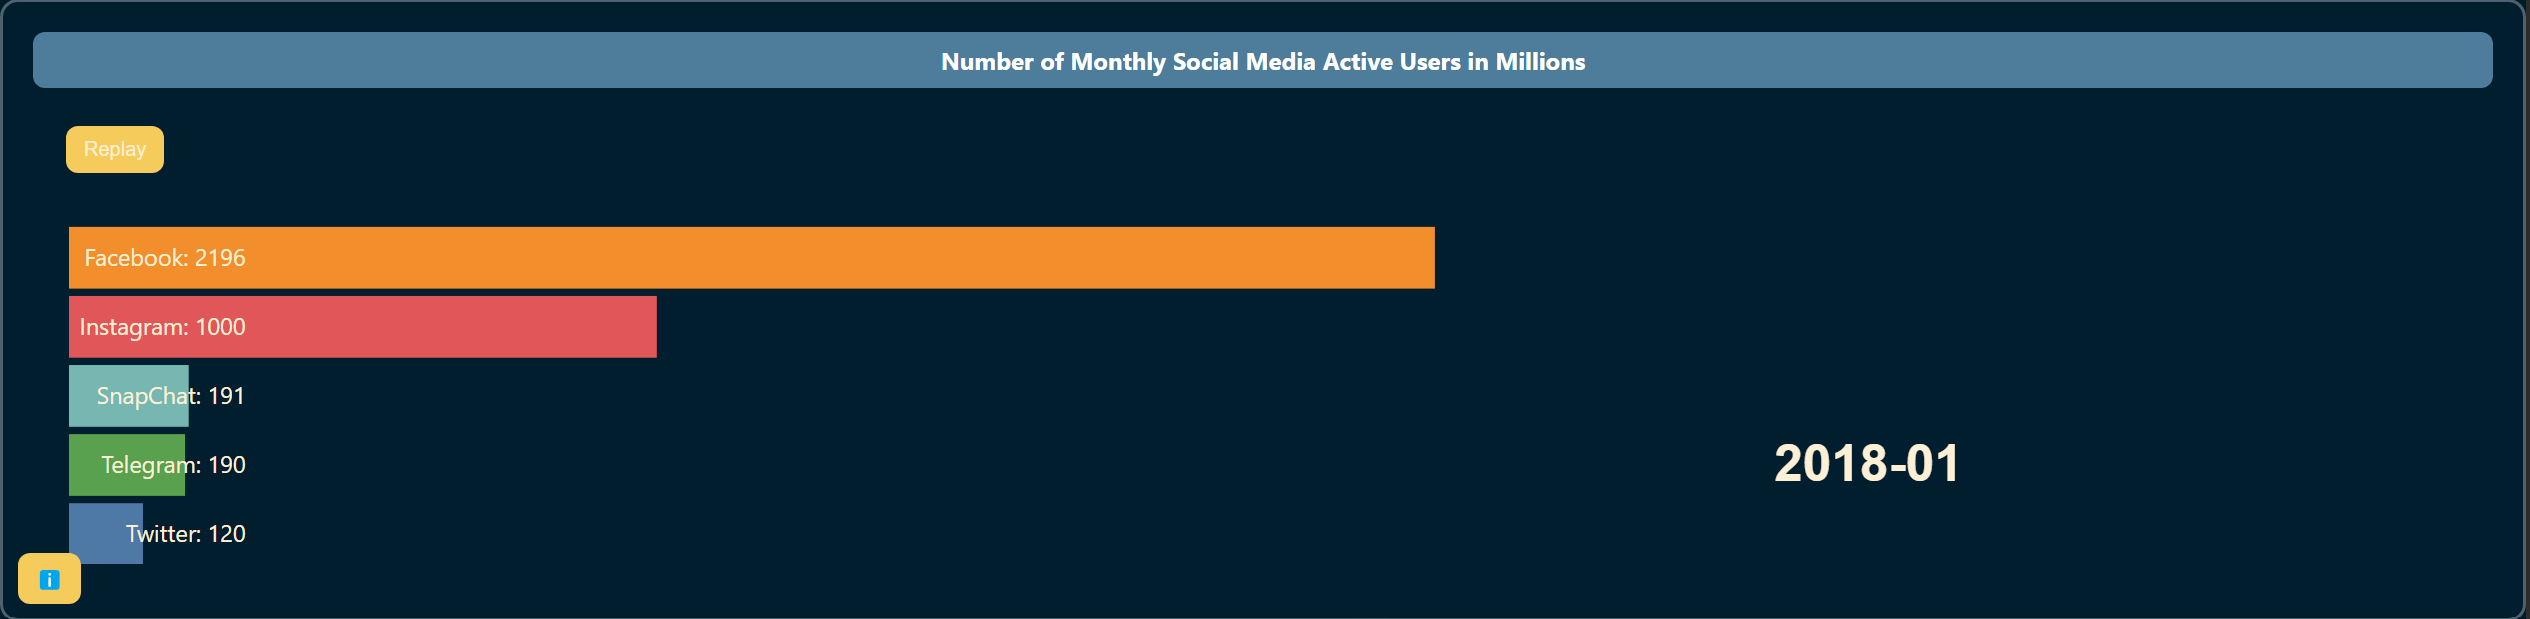
\includegraphics[width=\textwidth]{ressources/barChartRace1.png}
\end{minipage}
\begin{minipage}{0.48\textwidth}
\centering
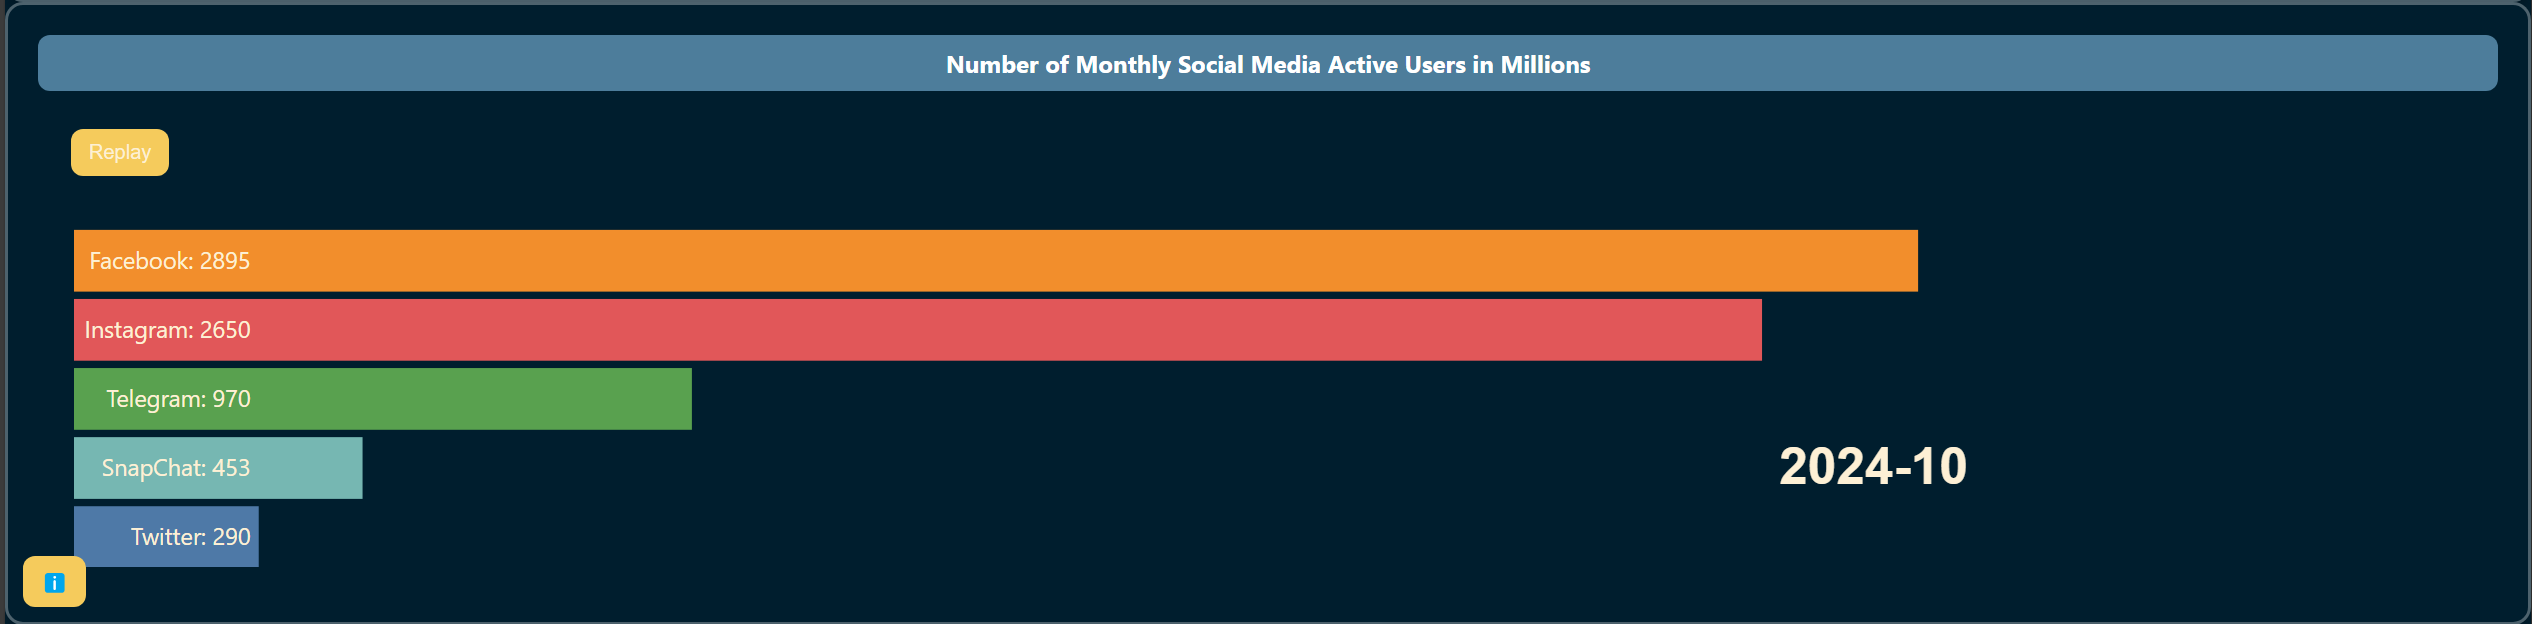
\includegraphics[width=\textwidth]{ressources/barChartRace2.png}
\end{minipage}
\caption{Number of Monthly Social Media Active Users in Millions}
\
\begin{minipage}{0.48\textwidth}
\centering
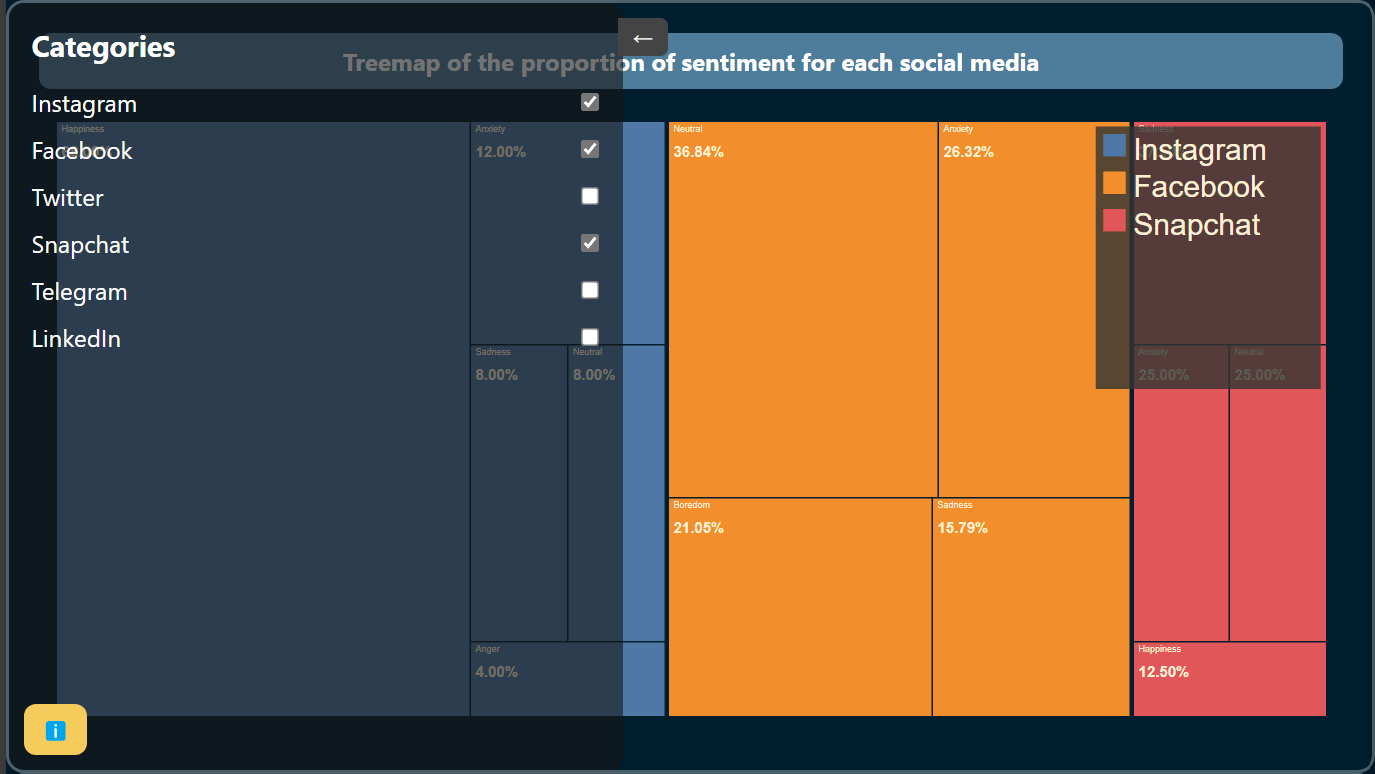
\includegraphics[width=\textwidth]{ressources/treeMap1.png}
\end{minipage}
\begin{minipage}{0.48\textwidth}
\centering
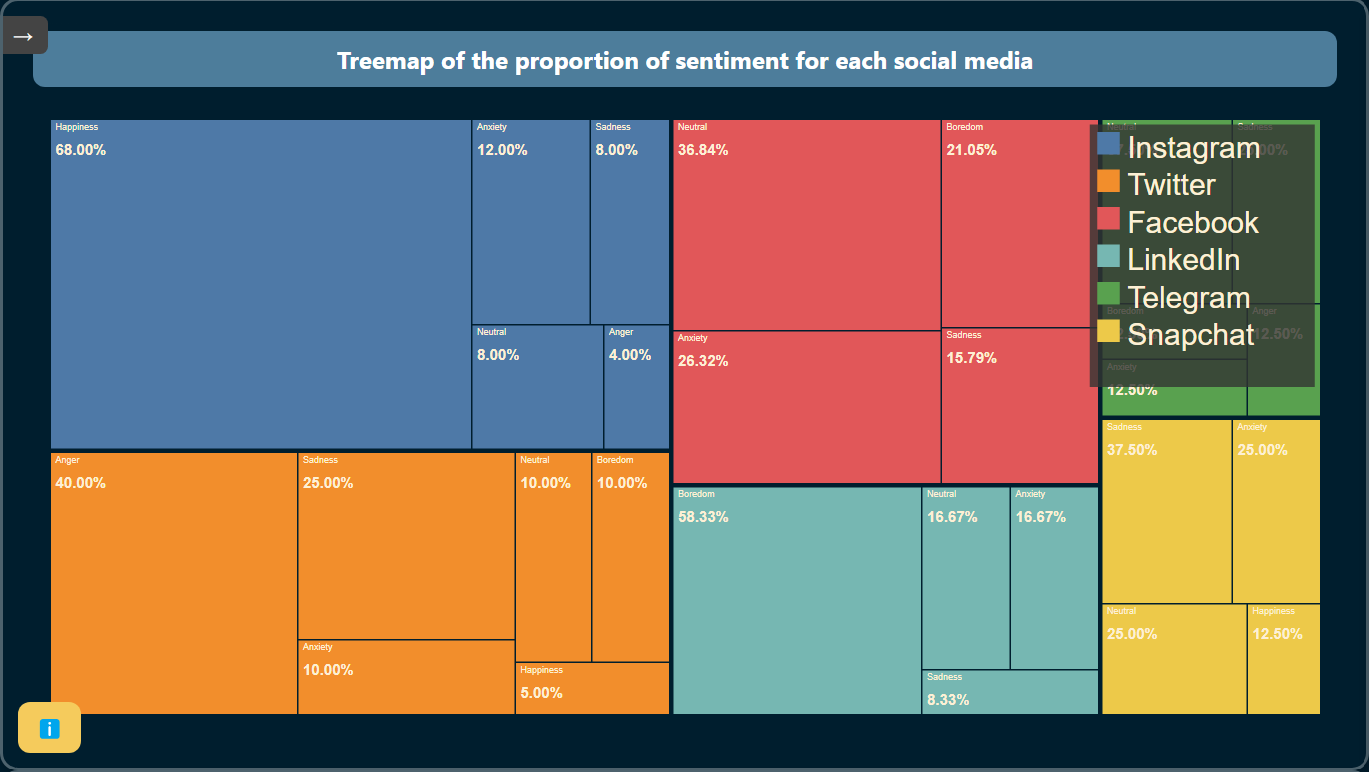
\includegraphics[width=\textwidth]{ressources/treeMap2.png}
\end{minipage}
\caption{Treemap of the proportion of sentiment for each social media}
\
\begin{minipage}{0.48\textwidth}
\centering
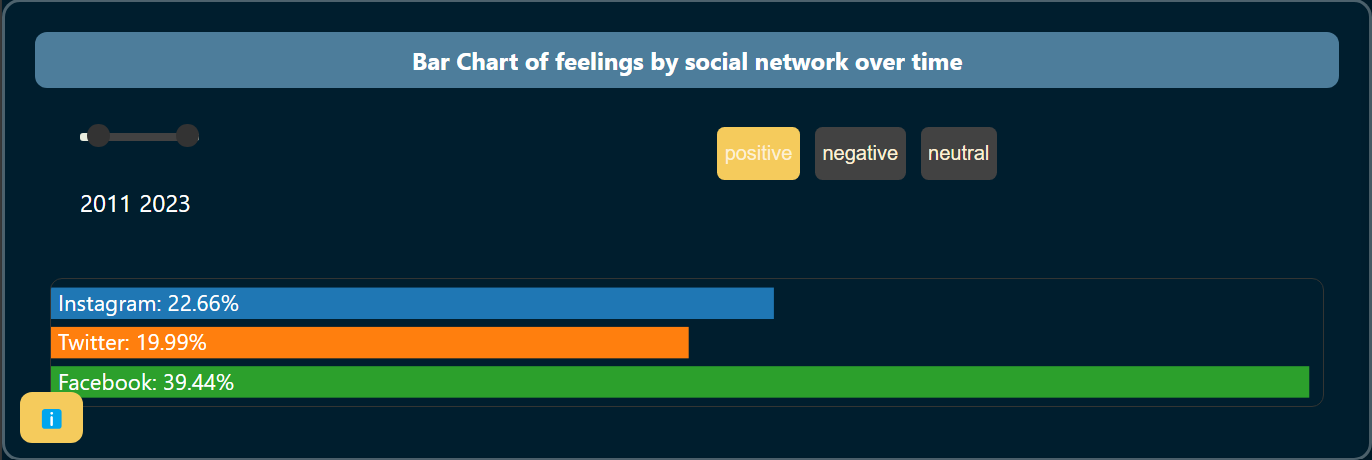
\includegraphics[width=\textwidth]{ressources/barChart1.png}
\end{minipage}
\begin{minipage}{0.48\textwidth}
\centering
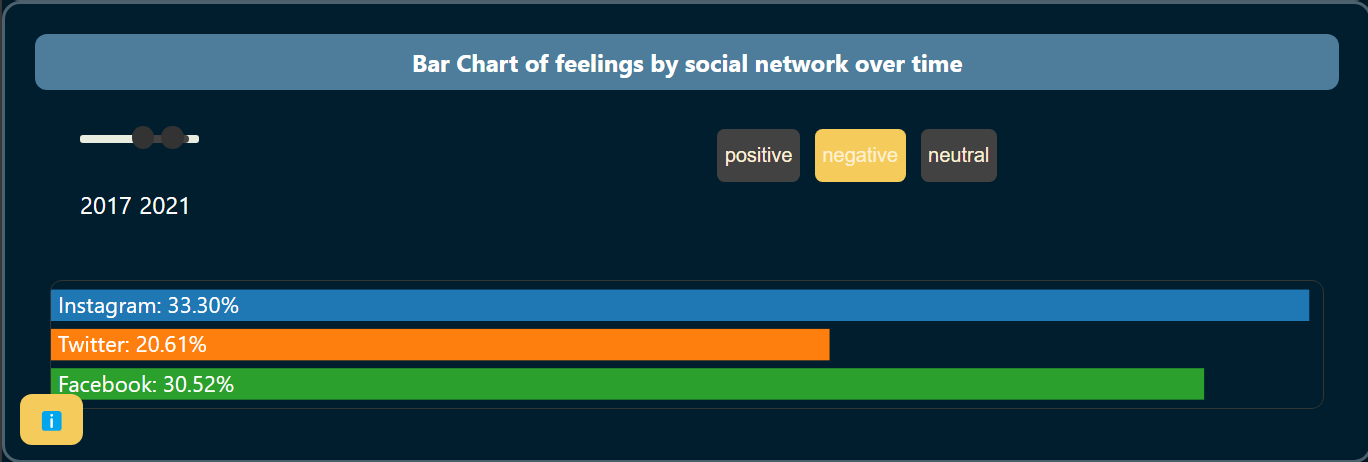
\includegraphics[width=\textwidth]{ressources/barChart2.png}
\end{minipage}
\caption{Bar Chart of feelings by social network over time}
\
\centering
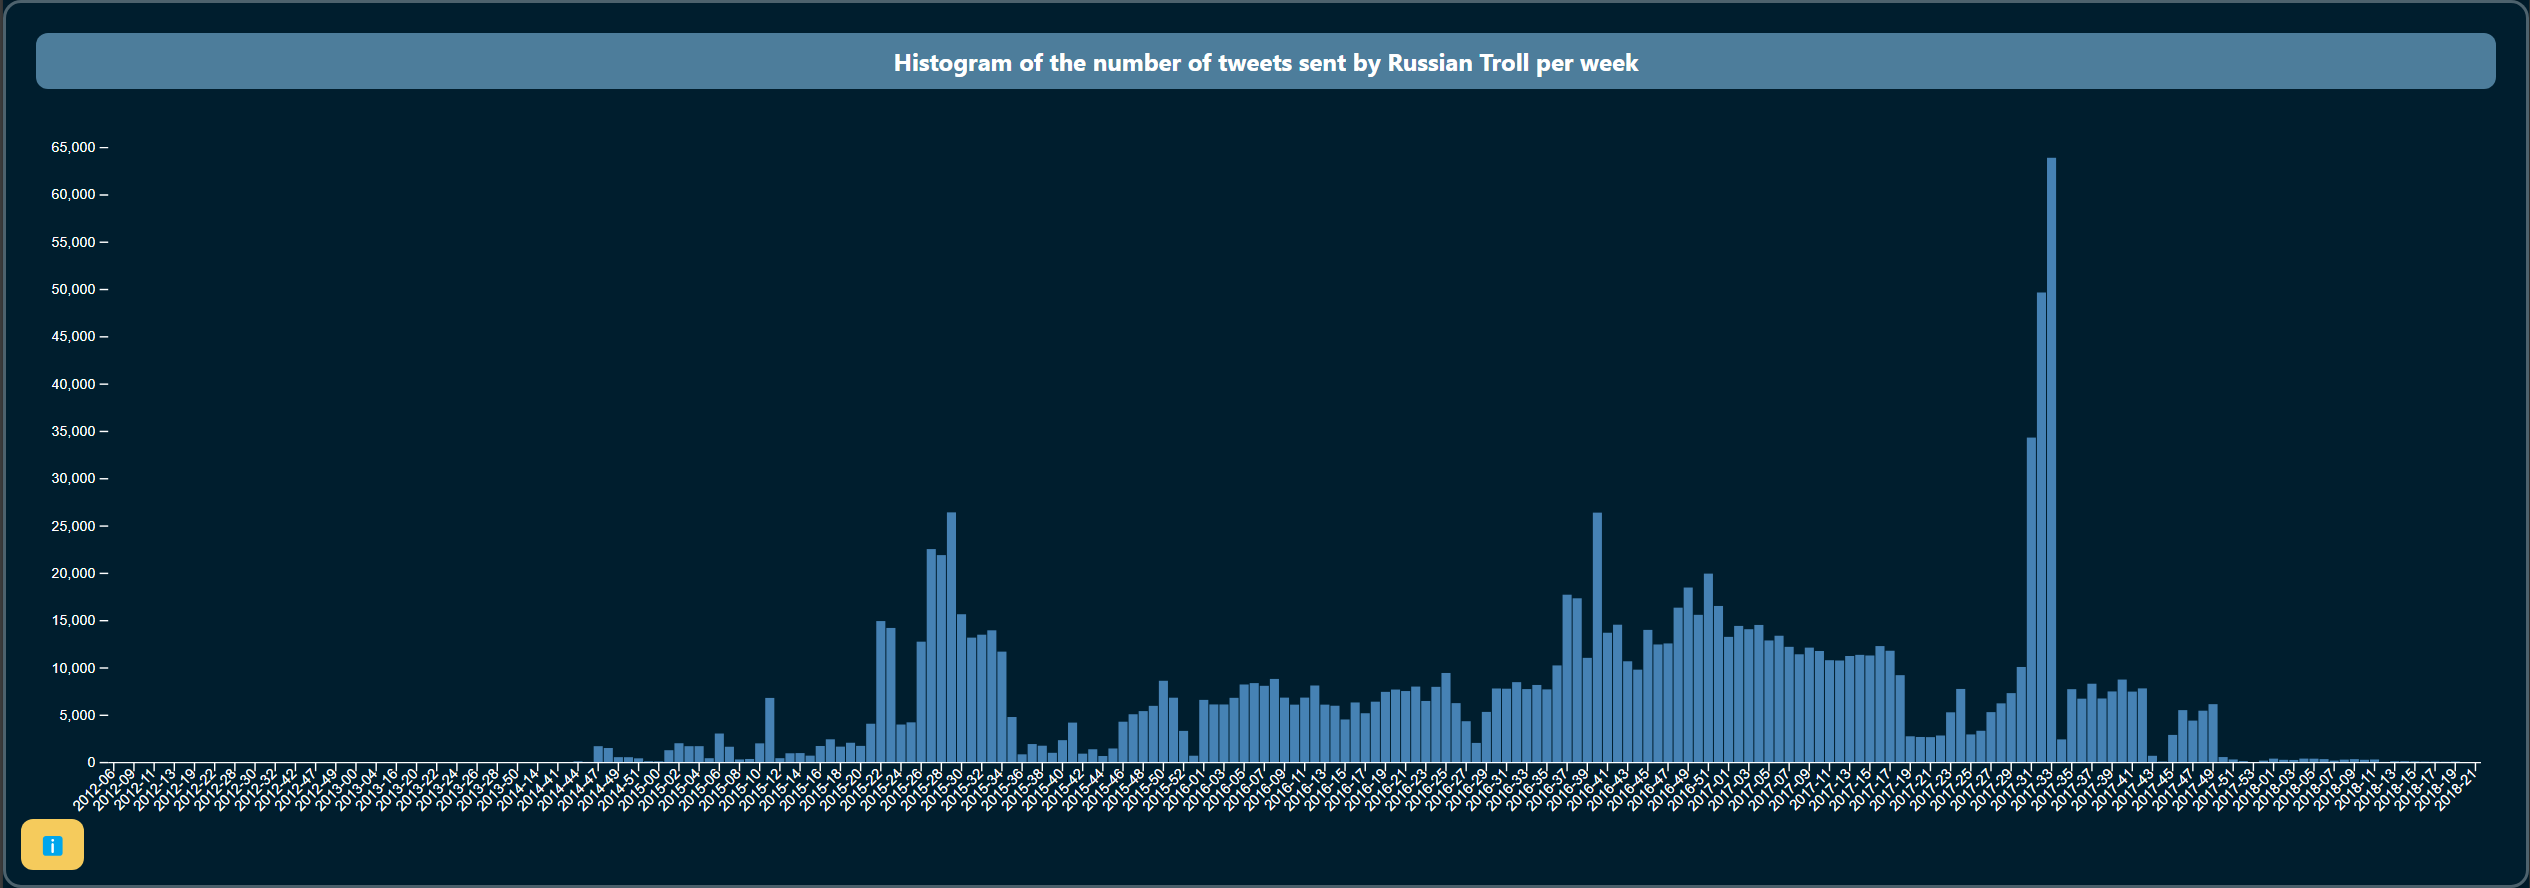
\includegraphics[width=0.75\textwidth]{ressources/histogram1.png}
\caption{Histogram of the number of tweets sent by Russian Troll per week}
\
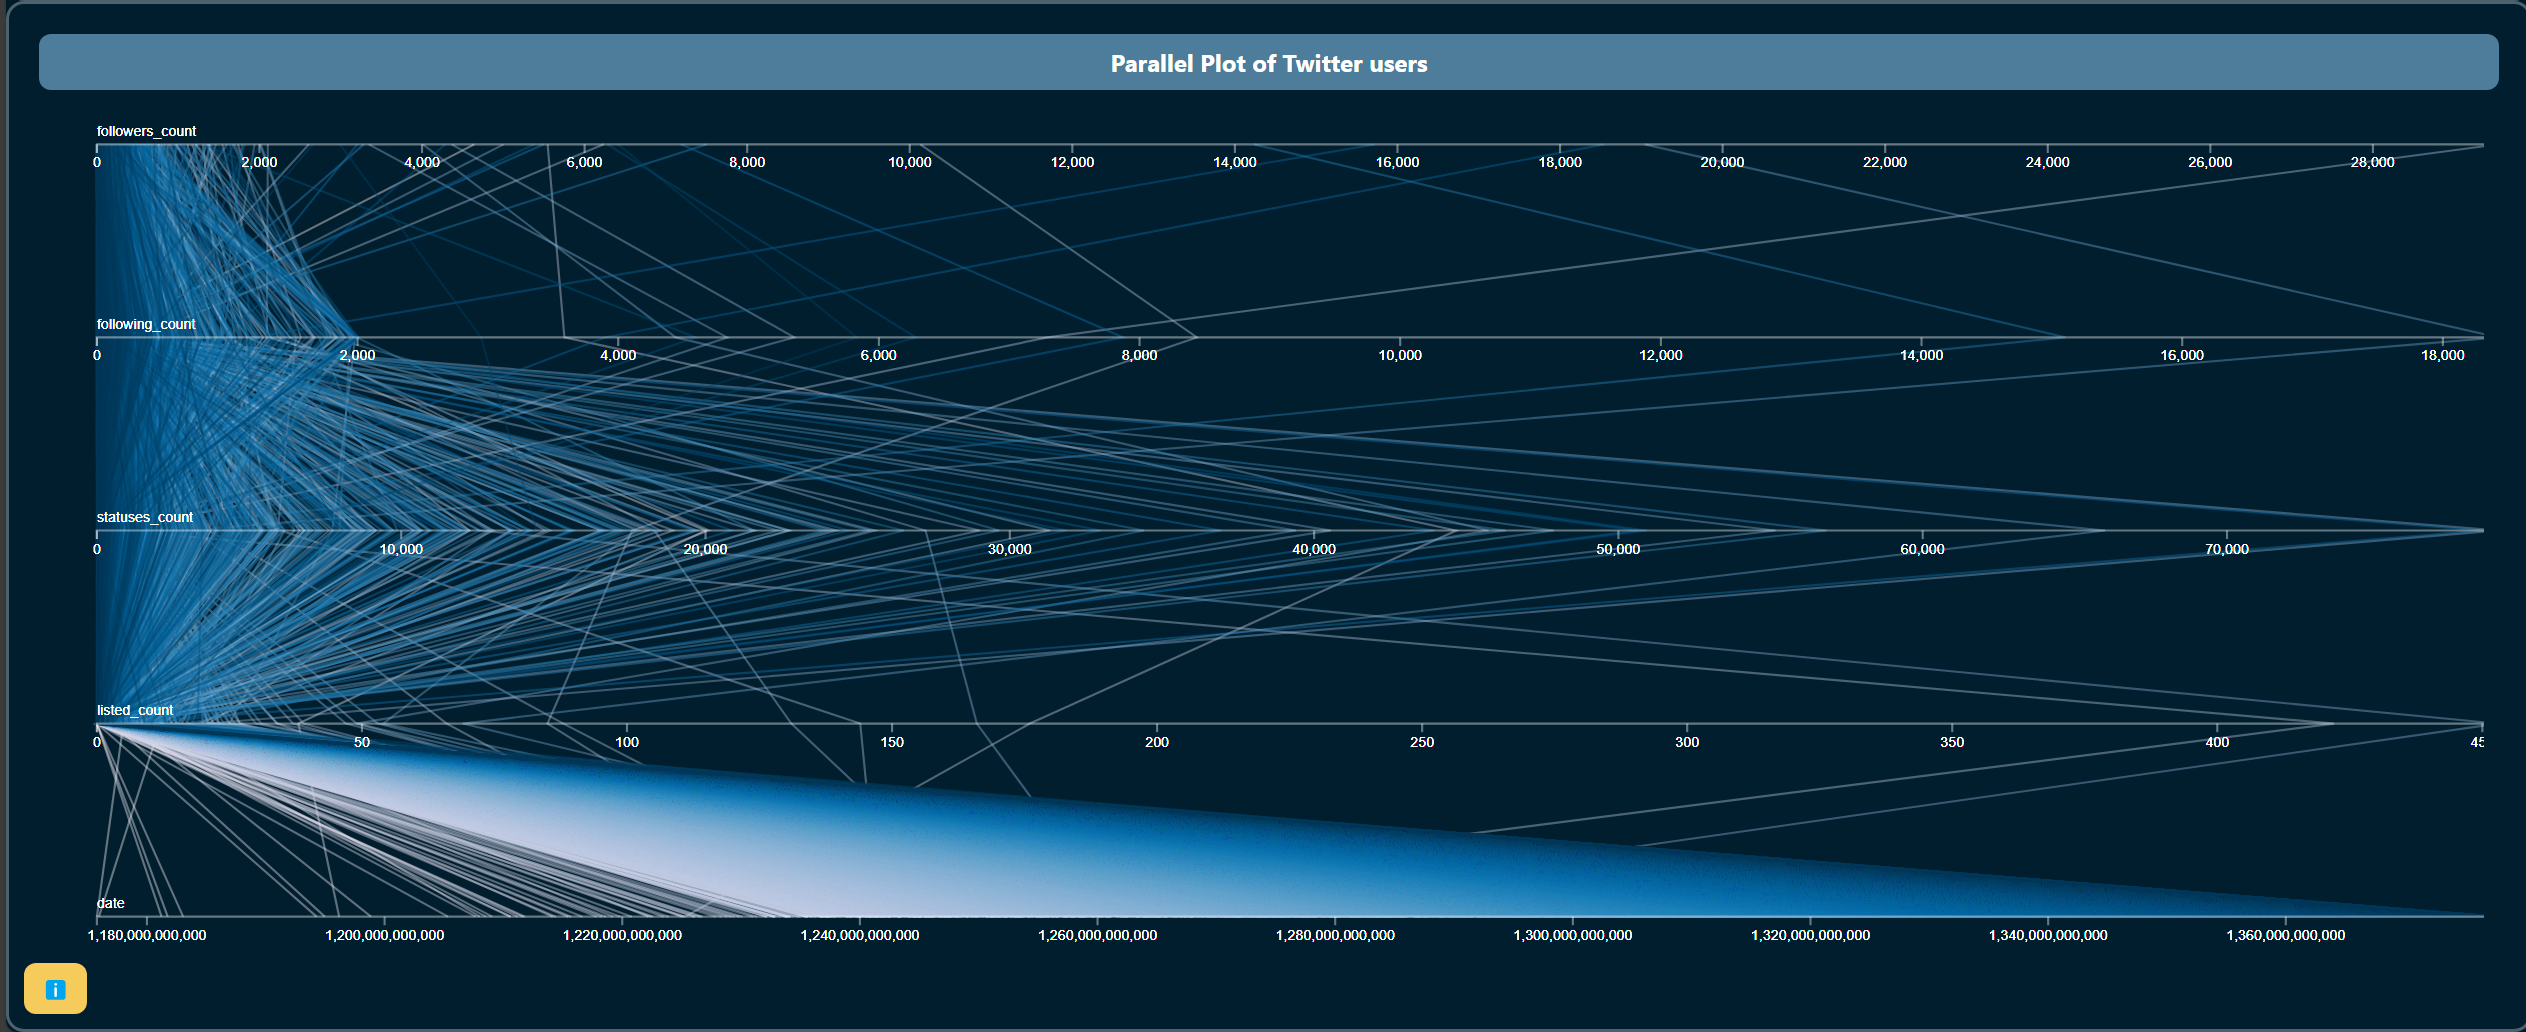
\includegraphics[width=0.75\textwidth]{ressources/parallelPlot.png}
\caption{Parallel Plot of Twitter users}
\end{figure}

\newpage
\section{Conclusion}
This project allowed me to deepen my knowledge of D3 and challenge myself with technical visualizations. I found the exercise of creating interconnected visualizations particularly interesting. Additionally, identifying appropriate and meaningful visualizations was not an easy task, especially considering the difficulty of finding datasets suited to the intended representations.

\begin{thebibliography}{9}
\bibitem{kaggle_facebook} Facebook. (2021). Monthly Active Users of Facebook [Data set]. Kaggle. \url{https://doi.org/10.34740/KAGGLE/DSV/2565605}
\bibitem{twitter_stats} X (Twitter) Statistics: How Many People Use X? (2025). \url{https://backlinko.com/twitter-users}
\bibitem{instagram_stats} How Many People Use Instagram 2025 (New Statistics). \url{https://www.demandsage.com/instagram-statistics/}
\bibitem{snapchat_stats} Snapchat Daily Active Users 2024. \url{https://www.statista.com/statistics/545967/snapchat-app-dau/}
\bibitem{telegram_stats} Telegram Global MAU 2024. \url{https://www.statista.com/statistics/234038/telegram-messenger-mau-users/}
\bibitem{kaggle_treemap} Emirhan BULUT. (2024). Social Media Usage and Emotional Well-Being [Data set]. Kaggle. \url{https://doi.org/10.34740/KAGGLE/DSV/8460631}
\end{thebibliography}



\end{document}
